        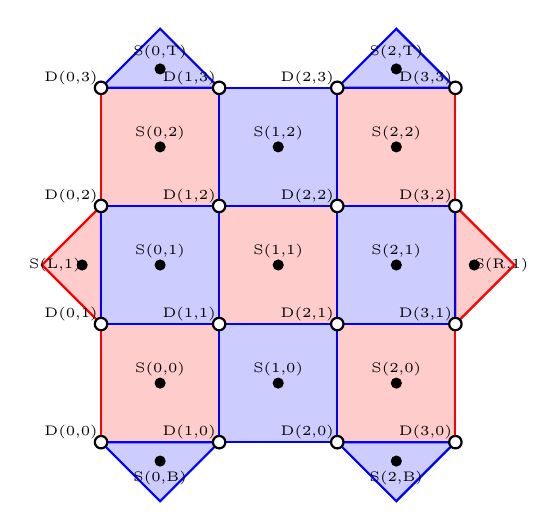
\begin{tikzpicture}[scale=1.5]
            % Z-stabilizers (Red full faces)
            \foreach \x/\y in {0/0, 2/0, 1/1, 0/2, 2/2} {
                \filldraw[red!20, draw=red, thick] (\x,\y) rectangle (\x+1, \y+1);
                \node[font=\tiny, inner sep=0.5pt] at (\x+0.5, \y+0.62) {S(\x,\y)};
            }
            
            % Z-stabilizers (Red half faces - Rough boundaries)
            \filldraw[red!20, draw=red, thick] (0,1) -- (0,2) -- (-0.5, 1.5) -- cycle; 
            \node[font=\tiny, inner sep=0.5pt] at (-0.39, 1.5) {S(L,1)};
            
            \filldraw[red!20, draw=red, thick] (3,1) -- (3,2) -- (3.5, 1.5) -- cycle; 
            \node[font=\tiny, inner sep=0.5pt] at (3.39, 1.5) {S(R,1)};
        
            % X-stabilizers (Blue full faces)
            \foreach \x/\y in {1/0, 0/1, 2/1, 1/2} {
                \filldraw[blue!20, draw=blue, thick] (\x,\y) rectangle (\x+1, \y+1);
                \node[font=\tiny, inner sep=0.5pt] at (\x+0.5, \y+0.62) {S(\x,\y)};
            }
            
            % X-stabilizers (Blue half faces - Smooth boundaries)
            \foreach \x in {0, 2} {
                \filldraw[blue!20, draw=blue, thick] (\x,0) -- (\x+1,0) -- (\x+0.5, -0.5) -- cycle;
                \node[font=\tiny, inner sep=0.5pt] at (\x+0.5, -0.3) {S(\x,B)};
                
                \filldraw[blue!20, draw=blue, thick] (\x,3) -- (\x+1,3) -- (\x+0.5, 3.5) -- cycle;
                \node[font=\tiny, inner sep=0.5pt] at (\x+0.5, 3.3) {S(\x,T)};
            }
        
            % Ancilla Qubits (Solid black dots, reduced size)
            \foreach \x/\y in {0.5/0.5, 2.5/0.5, 1.5/1.5, 0.5/2.5, 2.5/2.5, 1.5/0.5, 0.5/1.5, 2.5/1.5, 1.5/2.5} {
                \filldraw[black] (\x,\y) circle (1.2pt);
            }
            \filldraw[black] (-0.16, 1.5) circle (1.2pt);
            \filldraw[black] (3.16, 1.5) circle (1.2pt);
            \foreach \x in {0.5, 2.5} {
                \filldraw[black] (\x, -0.16) circle (1.2pt);
                \filldraw[black] (\x, 3.16) circle (1.2pt);
            }
        
            % Data Qubits (White circles, reduced size)
            \foreach \x in {0, 1, 2, 3} {
                \foreach \y in {0, 1, 2, 3} {
                    \filldraw[black, fill=white, thick] (\x,\y) circle (1.5pt);
                    \node[above left, font=\tiny, inner sep=1pt] at (\x,\y) {D(\x,\y)};
                }
            }
            
        \end{tikzpicture}
